% ----------------------------------------------------------------------- %
% Arquivo: cap2.tex
% ----------------------------------------------------------------------- %

% ----------------------------------------------------------------------- %
\chapter{Fundamentação Teórica}
\label{c_cap2}

O segundo capítulo (podendo ser desmembrado em mais capítulos) apresenta a revisão de literatura. Aqui, é importante que haja uma boa pesquisa bibliográfica para embasar todos os assuntos que você pretende desenvolver. 

Os níveis de abrangência e de profundidade da Fundamentação Teórica devem ser suficientes para evidenciar o conhecimento sobre o domínio da pesquisa. Porém, você deve focar no referencial teórico essencial para o trabalho. Lembre-se que, após a conclusão do trabalho, você deverá ter lido muito mais do que aquilo que foi colocado no texto. Ou seja, nem tudo que você precisa saber estará no texto. 

O capítulo não deve iniciar diretamente com uma seção (2.1, por exemplo). O início de cada capítulo deve apresentar uma breve discussão sobre o que será apresentado e por que este conteúdo é relevante para o entendimento do trabalho, ou seja, uma introdução ao capítulo.

A revisão da literatura deve ser complementada por um capítulo posterior (discutido mais a seguir), no qual deve ser descrito o estado da arte relacionado ao problema de pesquisa de modo a caracterizar a relevância desse problema e da solução proposta, posicionado-a em relação às soluções já desenvolvidas por outros pesquisadores.

O título do capítulo deve ser escrito com todas as letras em caixa alta (maiúsculas). As citações a capítulos ao longo do texto podem ser feitas das seguintes maneiras:

\begin{itemize}  
    \item ... no capítulo anterior;
    \item ... neste capítulo;
    \item ... no capítulo seguinte;
    \item ... o capítulo Fundamentação Teórica; ou
    \item ... o Capítulo 2.
\end{itemize}

Note que, quando você for identificar o capítulo pelo número, a palavra “Capítulo” deve iniciar com a letra “C” maiúscula, pois se trata da identificação do capítulo (essa mesma regra vale para subseções, figuras, tabelas e quadros). Nesse caso, para facilitar a edição do texto, procure utilizar o recurso de referência cruzada do editor1. Dessa forma, qualquer atualização feita no documento, poderá ser refletida automaticamente em todo o texto.



% ----------------------------------------------------------------------- %
\section{Exemplo de Título de Seção}
\label{s_c2_exemplo01}

Cada capítulo do texto pode ser dividido em seções (primeiro nível de subdivisão do capítulo), as quais devem ser usadas para separar os tópicos principais a serem abordados. Procure um equilíbrio entre as seções, evitando seções de tamanhos muito diferentes (ex. uma seção com uma ou duas páginas e outra com dez páginas). Seções muito longas podem até justificar um capítulo adicional próprio referente ao tema tratado na seção.

Uma seção pode ser dividida em até três níveis de subseção, dois deles numerados e um não numerado, conforme exemplificado logo a seguir. Evite o uso de subseções numeradas muito curtas (ex. com um ou dois parágrafos). Nesse caso, é preferível identificar a subseção usando o estilo não numerado.




% ----------------------------------------------------------------------- %
\subsection{Mais informações}
\label{ss_c2_mais-info}

Mais informações sobre quadros, tabelas, equações, etc, podem ser encontradas aqui: \url{http://www.univali.br/ensino/pos-graduacao/mestrado/mestrado-em-computacao-aplicada/formularios-e-modelos/Paginas/default.aspx}





% ----------------------------------------------------------------------- %
\section{Exemplo de Figura}
\label{ss_c2_exemplo-figura}

Uma figura é utilizada para apresentar gráficos, fotos, ilustrações, diagramas e qualquer outro material que não seja classificado como quadro ou tabela %\cite{oliveira:07}. 

As figuras inseridas no texto devem buscar um compromisso entre a qualidade gráfica o custo de armazenamento. Evite imagens com resolução muito baixa, que comprometam a qualidade visual, ou muito alta, que consumam muito espaço de armazenamento (em disco e na memória principal). Uma dica para reduzir a quantidade de memória consumida pelas figuras é colá-las como Imagem (Metarquivo do Windows) através do recurso de colar especial. A única restrição desse recurso é a perda do vínculo com o editor usado na composição da figura. Por isso, é recomendável manter todas as figuras usadas no texto numa pasta (diretório) de fácil acesso para possíveis atualizações.

Os textos das figuras devem ser legíveis. Recomenda-se o uso da fonte Arial (ou similar) com tamanho entre 6 e 12 (os tamanhos de 8 a 10 são os mais adequados). Dentro do possível, esses textos devem ser escritos em português. Por isso, evite copiar e simplesmente colar figuras escritas em outros idiomas. É sempre recomendável adaptar essas figuras traduzindo seus textos, ou, melhor ainda, redesenhando-as.

Quando o espaço disponível em uma folha A4 for insuficiente para assegurar a qualidade visual da figura, é recomendável imprimi-la em uma folha A3.

A seguir, é ilustrado um exemplo de figura (\autoref{f_modelos_SGId}) que deve ser utilizado como referência. Note que a figura é emoldurada por uma borda fina e suas legendas e a fontes de referência aparecem abaixo da figura. Esse conjunto todo é ainda emoldurado iagual a uma célula de tabela sem borda, a qual é utilizada para evitar que esses elementos sejam apresentados em páginas diferentes quando uma figura é posicionada na parte inferior da página. 


% Figura - Classificação dos Modelos de SGId
\begin{figure}[!htpb]
  \centering
  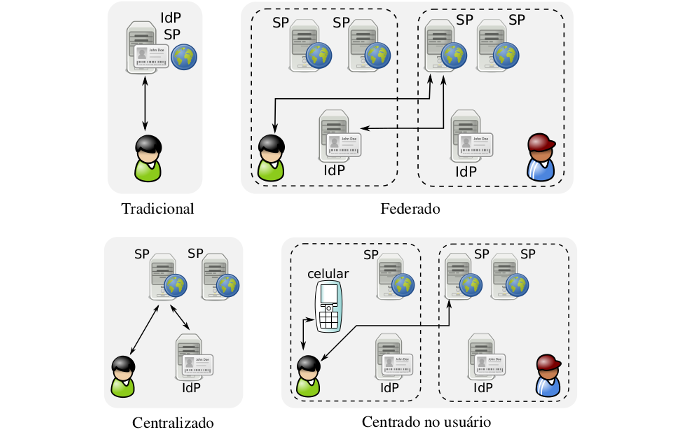
\includegraphics[width=.89\linewidth,fbox]{figs/Modelos_SGId.png}
  \caption{Classificação dos modelos de gerenciamento de identidade}
  \raggedright Fonte: Adaptado de %\citeonline{wangham:10}.
  \label{f_modelos_SGId}
\end{figure}



% ----------------------------------------------------------------------- %
\section{Exemplo de Tabela}
\label{ss_c2_exemplo-tabela}

%Uma tabela normalmente apresenta resultados quantitativos (números) e é usada para apresentar dados primários %\cite{oliveira:07}. Geralmente está presente em seções referentes aos resultados e do trabalho. Nada impede, porém, que uma tabela seja usada na fundamentação teórica.

A identificação da tabela é feita por uma legenda e por um título, separados por ponto, sendo que não se coloca o ponto final de parágrafo no final do título (conforme mostrado nos exemplos).

Quanto à formatação do seu conteúdo, podem ser usados espaçamento e fontes de letras com tamanhos menores que o do texto (não precisa seguir o mesmo padrão). Se o texto usa fonte 12, a tabela pode ser feita em fonte 11 ou 10.

Quando uma tabela for baseada em dados publicados em outro trabalho, a fonte de referência deve ser citada logo abaixo da tabela obedecendo às normas da ABNT4, indicando os autores do trabalho consultado e o ano da publicação do trabalho (entre parênteses),

\begin{table}[!htbp]
\begin{center}
\begin{footnotesize}
\caption{Exemplo de Tabela: Extração e Análise dos Dados - RSL 02}
\label{t_apendiceC-rsl}

\begin{tabular}{l|c|c|c|c|c|c|}
\cline{2-7}
 & \textbf{ACM} & \textbf{IEEExplore} & \multicolumn{1}{l|}{\textbf{ScienceDirect}} & \textbf{Scopus} & \textbf{Springer} & \textbf{Total de artigos} \\ \hline
\multicolumn{1}{|l|}{\textbf{Resultado da \textit{string} de busca}} & 24 & 26 & 9 & 49 & 154 & 262 \\ \hline
\multicolumn{1}{|l|}{\textbf{Trabalhos repetidos}} & 7 & 1 & 7 & 22 & 0 & 37 \\ \hline
\multicolumn{1}{|l|}{\textbf{Trabalhos removidos}} & 15 & 20 & 2 & 21 & 153 & 211 \\ \hline
\multicolumn{1}{|l|}{\textbf{Trabalhos pré-selecionados}} & 2 & 5 & 0 & 6 & 1 & 14 \\ \hline
\multicolumn{1}{|l|}{\textbf{Trabalhos aceitos}} & 1 & 1 & 0 & 2 & 0 & 4 \\ \hline
\end{tabular}

\end{footnotesize}
\end{center}
\raggedright Fonte: Elaborada pelo próprio autor.
\end{table}



% ----------------------------------------------------------------------- %
\section{Considerações}
\label{s_c2_consideracoes}

Texto das considerações do capítulo.
